% Interaction-led recomposition of the implemented console and saved evidence.
% Native size 178 x 154 mm. Charts and prefix lengths remain proportional.
% Qwen3-4B interaction/inspector: live-run.json, saved November 8.
% Qwen3-30B AgentX capacity comparisons: paper-evidence.json.
% The inspector overlaps reserved whitespace, not request content or data.
% Its status is a clipped, unmodified native screenshot. The popup-like layout
% is a presentation enlargement, not a claim that the UI implements a modal.
\usetikzlibrary{patterns}
\begingroup
\definecolor{viewInk}{HTML}{222222}
\definecolor{viewRaw}{HTML}{707070}
\begin{tikzpicture}[x=1cm,y=1cm,text=viewInk,
  font=\fontsize{10.5}{12}\selectfont,line cap=round,line join=round,
  every node/.style={inner sep=0pt},
  title/.style={font=\fontsize{12}{14}\selectfont\bfseries},
  note/.style={font=\fontsize{9.5}{11}\selectfont},
  label/.style={font=\fontsize{10.5}{12}\selectfont\bfseries},
  metric/.style={font=\fontsize{11.5}{13}\selectfont\bfseries},
  control/.style={draw=viewInk!45,fill=white,rounded corners=1.5pt,
    minimum height=.50cm,font=\fontsize{10.5}{12}\selectfont},
  flow/.style={-{Stealth[length=1.5mm,width=1.2mm]},line width=.75pt}]
  \path[use as bounding box] (0,0) rectangle (17.8,15.4);

  % (a) A front-facing console window: controls, input, reuse, and answer.
  \draw[viewInk!55,fill=white,rounded corners=2pt,line width=.65pt]
    (.05,5.70) rectangle (16.95,15.35);
  \fill[fpBlue!6,rounded corners=2pt] (.07,14.65) rectangle (16.93,15.33);
  \draw[viewInk!25,line width=.5pt] (.05,14.65) -- (16.95,14.65);
  \node[title,anchor=west] at (.35,15.00) {(a) Prefix reuse};
  \node[note,anchor=east] at (16.60,15.00) {Saved interaction};
  \foreach \x/\label in {2.25/{1. Build},6.35/{2. Append},10.45/{3. Edit early},14.55/{4. Restore}} {
    \node[control,minimum width=3.70cm] at (\x,14.13) {\label};
  }

  % Exact excerpts; line breaks are for paper width, not changed prompt text.
  \draw[viewInk!22,fill=viewInk!2,rounded corners=1.5pt,line width=.5pt]
    (.40,10.08) rectangle (7.55,13.60);
  \node[label,anchor=west] at (.65,13.26) {Prompt excerpt};
  \node[anchor=north west,align=left,font=\fontsize{9.5}{11.3}\selectfont\ttfamily]
    at (.65,12.91) {You are maintaining a Python\\
      repository. Diagnose the timeout\\
      failure below.};
  \node[anchor=north west,align=left,font=\fontsize{9}{11}\selectfont\ttfamily]
    at (.65,11.51) {deadline = monotonic() + timeout\\
      connection = await client.acquire()};

  \node[label,anchor=west] at (7.95,13.35) {Reused / prompt tokens};
  \foreach \x/\col/\lab in {7.95/fpTeal/Reused,10.67/fpBlue/Restored,13.66/fpOrange/Computed} {
    \fill[\col!85] (\x,12.85) rectangle +(.16,.16);
    \node[note,anchor=west] at (\x+.24,12.93) {\lab};
  }
  % One shared 656-token scale; completed steps are a trace, not an animation.
  \foreach \y/\lab/\total/\reuse/\col in {
    12.28/Build/534/0/fpTeal,
    11.63/Append/656/512/fpTeal,
    10.98/{Edit early}/534/0/fpTeal,
    10.33/Restore/534/512/fpBlue} {
    \node[note,anchor=west] at (7.95,\y) {\lab};
    \fill[viewInk!5] (10.05,\y-.13) rectangle +(4.43,.26);
    \draw[fpOrange!80,fill=fpOrange!65,line width=.4pt]
      (10.05,\y-.13) rectangle +({4.43*\total/656},.26);
    \ifnum\reuse>0
      \draw[\col,fill=\col!80,line width=.4pt]
        (10.05,\y-.13) rectangle +({4.43*\reuse/656},.26);
    \fi
    \foreach \k in {1,2,3,4} {
      \draw[white,line width=.6pt] ({10.05+4.43*128*\k/656},\y-.13) -- +(0,.26);
    }
    \node[label,anchor=east] at (16.60,\y) {\reuse\,/\,\total};
  }

  % The rightmost blank part of this panel lies behind the inspector.
  \draw[viewInk!22,fill=white,rounded corners=1.5pt,line width=.5pt]
    (.40,6.02) rectangle (12.05,9.65);
  \node[label,anchor=west] at (.65,9.31) {Model response};
  \node[note,anchor=east,text=fpBlue] at (10.82,9.31) {Restore};
  \node[anchor=north west,text width=9.80cm,align=left,
    font=\fontsize{10.5}{13}\selectfont] at (.65,8.88)
    {The root cause is that the \texttt{timeout} parameter is only used to
    set a deadline for the function's execution, but it is not enforced
    during the \texttt{client.acquire()} call.};
  \draw[viewInk!15,line width=.4pt] (.65,7.02) -- (10.82,7.02);
  \node[anchor=west] at (.65,6.63) {\textbf{512} reused tokens};
  \node[anchor=west] at (4.60,6.63) {TTFT \textbf{47.3 ms}};
  \node[note,anchor=east] at (10.82,6.63) {DRAM $\rightarrow$ GPU};

  % Enlarged independent inspector. This is not a Restore verification path.
  \fill[viewInk!10,rounded corners=2pt] (11.56,5.62) rectangle (17.78,9.97);
  \draw[fpTeal!75,fill=white,rounded corners=2pt,line width=.75pt]
    (11.43,5.75) rectangle (17.65,10.10);
  \fill[fpTeal!7,rounded corners=2pt] (11.45,9.48) rectangle (17.63,10.08);
  \draw[fpTeal!30,line width=.5pt] (11.43,9.48) -- (17.65,9.48);
  \node[title,anchor=west] at (11.70,9.79) {KV Inspector};
  \node[note,anchor=west] at (11.70,9.14) {Independent export/import check};
  \node[note,anchor=west] at (11.70,8.72) {Block 1 $\cdot$ 128 tokens $\cdot$ 36 layers};
  \node[note] at (12.67,8.25) {BF16};
  \node[note] at (15.69,8.25) {Encoded blob};
  \node[metric] at (12.67,7.83) {18.00 MiB};
  \draw[flow,fpTeal] (13.80,7.83) -- (14.50,7.83);
  \node[metric] at (15.69,7.83) {12.73 MiB};
  % Original native screenshot: viewport in pixels (= bp at its native 72 dpi).
  % Pixel rectangle [60,275,760,425], origin at the image's upper left.
  \node at (14.54,6.98) {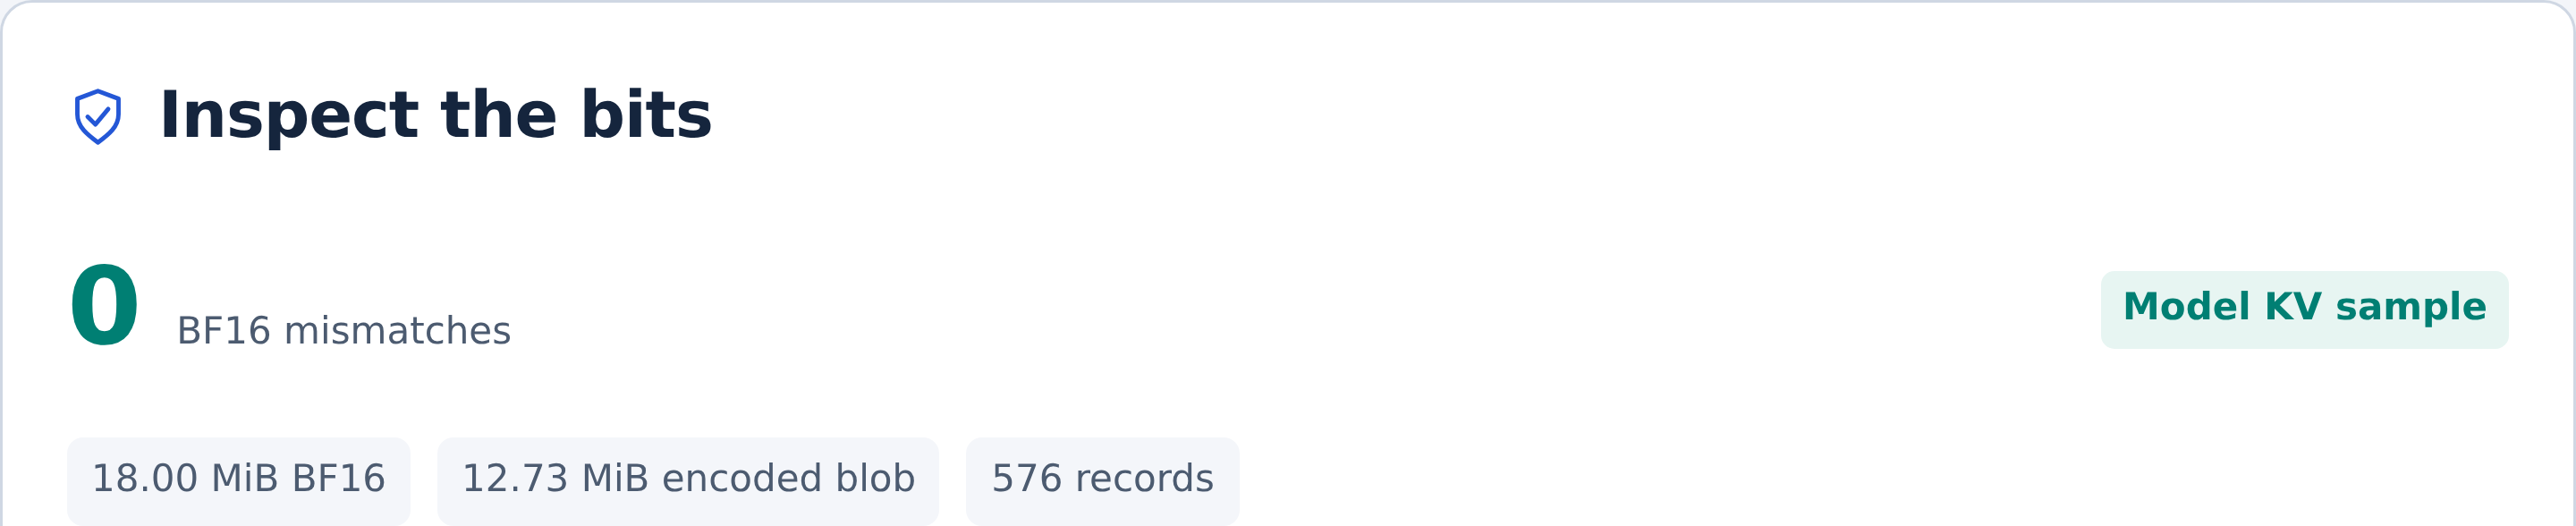
\includegraphics[viewport=60 163 760 313,clip,width=5.30cm]
    {images/console-inspector-recorded(9).png}};
  \node[note,anchor=west] at (11.70,6.12) {After Build $\cdot$ 576 records};

  % (b)(c) Compact, flat archive viewers: configuration and one central chart.
  \foreach \x in {.05,9.10} {
    \draw[viewInk!55,fill=white,rounded corners=2pt,line width=.6pt]
      (\x,.08) rectangle +(8.65,5.05);
  }
  \node[title,anchor=west] at (.35,4.75) {(b) GPU capacity};
  \node[note,anchor=east,text=viewRaw] at (8.40,4.75) {Recorded};
  \node[anchor=west] at (.35,4.11) {Admission};
  \node[control,minimum width=1.45cm] at (5.12,4.11) {$S=8$};
  \node[control,draw=fpBlue,fill=fpBlue!7,minimum width=1.65cm]
    at (7.35,4.11) {$S=12$};
  \node[label,anchor=west] at (.35,3.48) {KV tokens / GPU};
  \node[note,anchor=east] at (8.40,3.48) {54 GiB budget};
  \foreach \y/\lab/\val/\disp/\col in {
    2.82/Raw/1.18/1.18M/viewRaw,2.19/Pool/1.59/1.59M/fpBlue} {
    \node[anchor=west] at (.35,\y) {\lab};
    \fill[viewInk!4] (1.65,\y-.15) rectangle +(5.15,.30);
    \draw[\col,fill=\col!20,line width=.6pt]
      (1.65,\y-.15) rectangle +({5.15*\val/1.6},.30);
    \node[metric,anchor=east] at (8.40,\y) {\disp};
  }
  \draw[viewInk!15,line width=.4pt] (.35,1.67) -- (8.40,1.67);
  \node[note,anchor=west] at (.35,1.19) {Waiting requests (mean)};
  \node[anchor=east] at (8.40,1.19) {1.5 $\rightarrow$ \textbf{0.4}};
  \node[note,anchor=west] at (.35,.61) {Engine TTFT (s)};
  \node[anchor=east] at (8.40,.61) {5.16 $\rightarrow$ \textbf{1.94}};

  \node[title,anchor=west] at (9.40,4.75) {(c) History retention};
  \node[note,anchor=east,text=viewRaw] at (17.45,4.75) {Recorded};
  \node[anchor=west] at (9.40,4.11) {NVMe};
  \node[control,draw=fpTeal,fill=fpTeal!7,minimum width=1.95cm]
    at (13.75,4.11) {640 GiB};
  \node[control,minimum width=1.65cm] at (16.35,4.11) {2 TiB};
  \node[label,anchor=west] at (9.40,3.48) {Cached tokens (GPU + external)};
  \foreach \y/\lab/\val/\col in {2.82/Raw/55/viewRaw,2.19/Tier/91/fpTeal} {
    \node[anchor=west] at (9.40,\y) {\lab};
    \fill[viewInk!4] (10.70,\y-.15) rectangle +(5.15,.30);
    \draw[\col,fill=\col!20,line width=.6pt]
      (10.70,\y-.15) rectangle +({5.15*\val/100},.30);
    \node[metric,anchor=east] at (17.45,\y) {\val\%};
  }
  \draw[viewInk!15,line width=.4pt] (9.40,1.67) -- (17.45,1.67);
  \node[note,anchor=west] at (9.40,1.19) {Stored / raw bytes};
  \node[anchor=east] at (17.45,1.19) {\textbf{71.6\%}};
  \node[note,anchor=west] at (9.40,.61) {Engine TTFT (s)};
  \node[anchor=east] at (17.45,.61) {6.76 $\rightarrow$ \textbf{2.34}};
\end{tikzpicture}
\endgroup
